% !TeX spellcheck = es_ES
\chapter{Palabras nuevas}


% Intro {{{

En el capítulo anterior se mencionó que el algoritmo toma como  idioma
dominante a aquel que transmite palabras hacia los demás y que estas perduran en los receptores al menos dos años.  El movimiento de palabras, es una característica que puede proporcionar información sobre la influencia entre los idiomas, sin embargo  puede resultar ambiguo decir que algo es más o menos influyente, además  no existe en la literatura un método que mida la influencia.

%El empleo de estás características puede proporcionar información acerca de la influencia que ejercen los idiomas,  sin  embargo, establecer un método que brinde un resultado al cual ligar la expresión influencia  no es sencillo, no existe en la literatura tal proceso, además puede ser ambiguo decir que algo es más o menos influyente sin un valor que lo respalde

\cpnote{Esta frase esta muy muy confusa. Simplifica por favor.}
\jmnote{Listo}

%Al momento, en la literatura no existe una serie de pasos a seguir cuyo resultado final sea una cantidad que mida la influencia. Para llegar a esta resolución se requieren establecer nuevas condiciones en la base de datos, y a partir de ellas trazar posibles caminos que lleven a relaciones y resultados  con los cuales satisfacer una interpretación de la influencia

%\fxnote{ah? Otra palabra que no cuadra para nada\ldots}, 
%\fxnote{No  entiendo la ultima frase. Ten cuidado con los cambios. Siento que lo intentas hacer un poco rococo y elegante, pero por tratar, pierdes precision. Creo qeu lo mas importante  en textos cientificos es ser preciso, ordenado y conciso.}.


% \fxnote{division? No entendi\ldots}
% \fxwarning{deje comentado el texto donde me dejaste la nota y lo cmabie por el siguiente} 
% 
% \fxwarning{Ya trate de ser más conciso en lo que quiero decir, corregi todo el parrafo}
% 



%\fxnote{Revisa redaccion} 
%\fxwarning{listo}
 

%El llegar a esta conclusión requiere el establecer condiciones y características en los elementos para poder llegar a un resultado que satisfaga una interpretación de la influencia. 

%\fxnote{Frase hueva. Que paso??? Se te bajo mucho el nivel de escritura}.
%\fxwarning{Listo, la corregi, comentare todas las frases o parrafos que vaya corrigiendo, para notar si hay un cmabiuo en la calidad}
 

% \fxnote{Ya no entiendo que quieres lograr con el siguietne parrafo. No se cual es el mensaje principal. De nuevo ``teñir un panorama'' no me suena correcto. Hablemos de la estructura de un parrafo y creo que tocara iterar de neuvo!!! Argh.}
% \fxwarning{ya Corregí todo el ,  dejo comentado el parrafo viejo}

%Aludiendo al capítulo  anterior, el tratamiento de la base de datos brinda información de los orígenes, los receptores y las palabras que migran de un lado a otro; comenzando con estos elementos, un primer paso es identificar los tiempos donde ocurren las migraciones. Antes de comprometer completamente al tiempo, es conveniente hacer una clasificación dentro de los propios préstamos para teñir un panorama más claro con el cual trabajar. 

Un primer paso para llegar a un valor que cuantifique a la influencia, es estudiando los tiempos donde ocurren las migraciones, encontrando relaciones entre dichos tiempos y las palabras involucradas en el movimiento. Antes de profundizar en esta idea, es conveniente realizar una clasificación dentro los préstamos,  para trabajar sobre ella y llegar a la cuantificación. 

Si se tiene una pareja de idioma origen \textit{A} e idioma receptor
\textit{B},  dentro de los préstamos de \textit{A} en \textit{B} se definen
como  \textbf{préstamos nuevos} a las  palabras que aparecen por primera vez en
las más usadas del idioma \textit{B}. Esta definición permite ordenar a los
préstamos nuevos por cada pareja de origen y receptor, y dentro  de este
ordenamiento, una segunda organización  por el año en el cual aparecieron. 



Dada la nueva clasificación, se determinaron tres posibilidades con las cuales interpretar influencia de un idioma sobre otro,  estas son: 

\begin{enumerate}
	\label{proceso.nuevos}
	
\item Contando por cada año los préstamos de origen \textit{A} que están presentes en los diferentes receptores; mostrando en cuales idiomas \textit{A} ha sido influyente.

\item Tomar ahora a \textit{A}  como el idioma receptor, y contando cuántos préstamos nuevos de diferentes orígenes están presentes cada año; obteniendo los idiomas que han influenciado a \textit{A}. 

\fxnote{El caso 1 y 2 no son equivalentes Mas bien el primero mide la influencia, y el punto dos la suceptibilidad.}
\fxwarning{Cierto, son diferentes, antes de las graficas puse como interpetar los dos puntos. }

\item Tomando fijos un idioma \textit{A} y un idioma \textit{B}, contabilizando cuántos préstamos nuevos por año se encuentran al tomar a  \textit{A} como origen y a \textit{B} como receptor,  una vez hecho esto,  repetir el conteo intercambiando a \textit{B} como el origen y a \textit{A} como el receptor. Obteniendo las épocas donde alguno de ellos tuvo más del punto uno o del dos. 

\end{enumerate}


%Las tres formas otorgan resultados diferentes,  el primer punto reflejará en que idiomas \textit{A} ha sido influyente, mientras que el segundo mostrará que tan susceptible es \textit{A} ante los demás idiomas,  finalmente el tercero combina la influencia con la susceptibilidad ya que al tratar únicamente a dos idiomas se verá en que épocas alguno de ellos ha tenido más del punto uno o del dos. }
\cpnote{Porfa revisa los parrafos. Por qué un parrafo tan largo?}
\jmnote{Listo, lo puse en los puntos anteriores ya que hablaba cual era el proposito de cada punto.}

% }}}
\section{Eventos que ayudan a las migraciones} % {{{

\cpnote{Otra vez veo frases innecesariamente largas. Porfa revisa todo el capitulo, y me avisas cuando hayas simplificado. Luego le sigues con el resto de la tesis. Una frase por idea, o por ahi dos, pero solo si tiene sentido. La siguiente frase hablas de dos cosas medio relacionadas, pero que seria mejor separar.}

\jmnote{Listo, ya corregí este parrafo}


Una parte complementaria de interpretar a la influencia es reconociendo causas que originan las migraciones. Por ejemplo, la globalización y el acceso al desarrollo tecnológico a finales de 1980 y principios de 1990, propició la migración  de términos como \textit{internet}, \textit{computadora}, \textit{web}, \textit{email} o \textit{software}, mostrando a ambos ámbitos como propagadores del movimiento de un grupo afín de palabras.

Las relaciones entre las causas y las migraciones serán identificables a partir  del significado de los préstamos involucrados en un año de migración,  ya que para un evento ocurrido en el mismo año (o en los años al rededor de él), las palabras migrantes pueden pertenecer a un mismo campo semántico relacionado al suceso.






%Una parte complementaria de interpretar la influencia es reconocer posibles causas que favorecen a las migraciones,  identificables por el tiempo donde ocurren, es decir, en un año de migración el significado de las palabras puede guardar alguna relación con un evento ocurrido durante el mismo año  (o en los años al rededor de él),  ya que las palabras migrantes pueden pertenecer a un mismo campo semántico relacionado al  evento. Por ejemplo, la globalización y el acceso al desarrollo tecnológico a finales de la década de 1980 y principios de 1990 propició la migración  de términos como \textit{internet}, \textit{computadora}, \textit{web}, \textit{email} o \textit{software}, mostrando a ambos ámbitos como propagadores del movimiento entre un origen y los distintos receptores. Al tratar con idiomas, se espera que en los eventos estén comprometidos países, personajes o comunidades que hablen o utilicen las lenguas involucradas. 

\fxnote{Cuando ocurrio la globalizacion y como se define? Es curioso, porque todos los ejemplos son cosas tecnollógicas asociadas con internet\ldots}

\fxwarning{Todas las palabras que mencione surgieron a partir de 1990. Puse este ejemplo porque pineso que la mayoria de personas puede conocer estos terminos y esta sumergida en estos ambitos, ademas  aceptan que se han mezclado con el español}











% }}}
\section{Palabras nuevas de un idioma en los demás} % {{{
 

Ya establecida la forma en que se buscarán  palabras nuevas en los diferentes idiomas,  los resultados encontrados se presentarán de la siguiente manera.

\begin{itemize}

\item Se buscaron los préstamos nuevos entre idiomas durante los 109 años comprendidos en el conjunto de búsqueda (1900-2009).
	
\item Por cada idioma se determinó la influencia que esté ejerció en los demás, mencionada en el punto 1 (ver pagina \pageref{proceso.nuevos}). La nomenclatura para la cantidad de palabras nuevas será $N_{p}$.

%\fxnote{Creo que hay forma de citar la pagina en cuestión. Debe ser un comando como ref o algo asi}. 
%\fxwarning{Ya lo corregí}
\fxnote{Si realmente las estas usando quiza valga la pena ponerle nombres a las cantidades, por ejemplo $F^{1954}_{\text{en} \to \text{fr}}$ ojala usando letras que tengan un significado, por ejemplo $S$ para susceptibilidad o como quieras llamarlo. } 
\fxwarning{listo}


\item En las graficas se mostrarán la cantidad de palabras que aparecieron en los 109 años y a la vez como se distribuye esta cantidad en las diferentes décadas. 

\item Se proporcionará en \cite{prestamos_nuevos} las listas  de préstamos nuevos entre cada pareja de origen y receptor, agrupados por el año de aparición .  Se especificará en \ref{lectura.listas}  la forma de leerlas.

\item En cada resultado y por cada par de idiomas se agregará un contexto  de los sucesos  que involucran a las migraciones. Esto permite omitir los resultados del punto 2 (ver  página \pageref{proceso.nuevos}), ya que muestra los campos donde \textit{A} influenció a  \textit{B}, y  de manera implícita los campos donde \textit{B} influenció a \textit{A}.

\item Los comentarios realizados estarán sustentados por la influencia entre \textit{A} y \textit{B}, (punto 3), las graficás correspondientes se anexaran en \ref{palabras.nuevas.apendice}. 

\end{itemize}

%\fxnote{Respecto al numero en la bibliografia despues de la referencia, para que lo quieres? Creo que no es estandard y a mi me confunde. Te propongo quitarlo.}

%\fxwarning{ok, veo como quitarlo por el momento no lo se}

\fxnote{No creo que amerite una subsección. La quite. Si no estas de acuerdo,  respondeme y la vuleves a poner.}

\fxwarning{de acuerdo, es más una adicion a la misma seccion}

Para las gráficas se utilizaron diferentes colores  y un sistema de abreviaciones para distinguir a los idiomas que intervienen, correspondiendo la primera abreviación al origen y la segunda al receptor. Los colores y abreviaciones de cada idioma se presentan  en la tabla \ref{tab.idcolor}. En todas las gráficas, el eje horizontal está representado por los años del conjunto de búsqueda 1900-2009,  mientras que en el eje vertical se presenta la
cantidad de prestamos nuevos $N_{p}$. 

%\fxnote{Nota como hace uno referencia a una tabla. Se deja flotante. Cuando  entiendas esta nota, borrala.}

\begin{table} % {{{
	\centering
	\begin{tabular}{ccc}
		\textbf{Idioma} & \textbf{Abreviación} & \textbf{Color} \\
		Inglés          & EN                   & Azul           \\
		Francés         & FR                   & Amarillo       \\
		Alemán          & GE                   & Violeta        \\
		Italiano        & IT                   & Verde          \\
		Español         & SP                   & Guinda        
	\end{tabular}
	\caption{Nomenclatura de los idiomas}
	\label{tab.idcolor}
\end{table} % }}}




\fxnote{Me parece que la anterior seccion y esta son una sola. Si quieres lo  discutimos}
	
\fxwarning{Cambie el nombre de la seccion por Palabras nuevas,  dentro de esta lo primero será especificar  como se presentan los resultados y las siguientes subsecciones los resultados mismos}

\fxnote{Antes de avanzar, tenemos que discutir las graficas. Creo que admiten una mejoría. Ver notas en un caption mas adelante y poner en espacio sencillo}

\fxwarning{listo}

\subsection{Inglés} % {{{

\begin{figure} % {{{
	\centering
	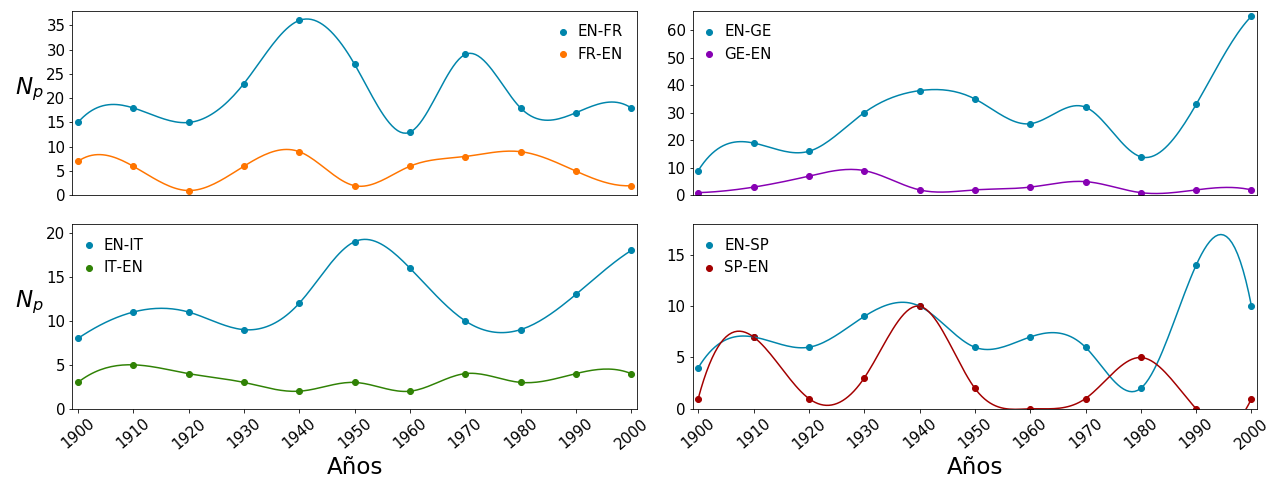
\includegraphics[scale=.38]{NC_EN.png}
	\label{fig.NC_EN}
	\caption{Palabras nuevas del inglés hacia los demás idiomas. El alemán se ha beneficado más del inglés, teniendo los mayores aportes en los primeros años del siglo XXI, caracterizado por palabras de tipo industrial y del desarrollo tecnológico.}
\end{figure} %  }}}

De manera general, el idioma que más se ha beneficiado del inglés ha sido el
alemán, con 300 préstamos en 100 años.  Inglés y alemán forman parte de la
misma familia lingüística de las lenguas germánicas,  posible razón de los
mayores intercambios. Entre las lenguas romances, el francés fue el más
favorecido, pero también es la más similar por las relación normanda entre
ambas.

\subsubsection*{Inglés-Francés} % {{{

Los mayores aportes se dieron de 1930 a 1970, periodo que engloba comienzos de
la gran depresión (1929), la segunda guerra mundial (1939-1945) y la guerra fría (1945-1991), sucesos donde
participaron países de ambas lenguas. Las palabras involucradas en este periodo
hacen referencia a estos eventos, entre 1944 y 1945 surgieron en el francés los
términos \textit{Churchill}, \textit{territories}, \textit{nazis} y
\textit{catastrophe},  mientras que  entre 1950 y 1970
aparecieron \textit{Nixon}, \textit{dollar} y \textit{Johnson}; dos de estas
palabras aluden a apellidos de presidentes de los Estados Unidos,  Lyndon B.
Johnson y Richard Nixon, cuyos periodos de gobierno fueron  entre 1963-1969 y
1969-1974 respectivamente.
% }}}
\subsubsection*{Inglés-Alemán} % {{{
Sólo  en dos de ellas (1900  y 1980) el alemán no fue el idioma que más prestamos recibió  del ingles. Entre las palabras encontradas
en las demás épocas están \textit{economic} (1929), \textit{depression} (1931),
\textit{investment} (1933), \textit{Roosevelt} (1935), que pertenecen al campo
semántico de la gran depresión mientras que el presidente Franklin D. Roosevelt
gobernó posterior a la crisis económica y durante la segunda guerra mundial. La crisis económica de la gran depresión, se origino en los Estados Unidos con consecuencias en diferentes países, entre ellos  Alemania, siendo uno de los motivos que propiciaron la segunda guerra mundial.

En las ultimas dos décadas, la globalización y  el desarrollo tecnológico son responsables del mayor aporte de palabras, entre ellas se encuentran \textit{standards} (1983),
\textit{market} (1994), \textit{internet} (1996), \textit{economy} (1996),
\textit{online} (1998), \textit{value} (2001), \textit{financial} (2003) y
\textit{customer} (2007). 
% }}}

\subsubsection*{Inglés-Italiano} % {{{
La principal característica de las palabras hacia el italiano son apellidos de personajes involucrados en la segunda guerra mundial, \textit{Roosevelt} (1941)
o \textit{Stalin} (1949), el  caso de Joseph Stalin a pesar de que su
nacionalidad no es la de algún pais de habla inglesa, en el ingles su apellido tomo notoriedad para exportarse a los otros idiomas; este es un ejemplo de que no todas las palabras encontradas surgieron en el idioma origen,  solamente en
el se hicieron populares.  En los últimos años nuevamente la globalización y la economia  han hecho favorable los préstamos del
ingles, \textit{internet} (1996), \textit{bussines} (2000), \textit{marketing}
(2001) y \textit{bush} (2002).


\subsubsection*{Inglés-Español} 
El español ha sido en cada década,  el idioma
que menos prestamos adopta del ingles, sin embargo los hechos a los que se
han ligado han sido en más áreas que en las otras combinaciones.  Nombres de organizaciones y empresas,  \textit{standard} (1933) (y \textit{oil} (1931) aludiendo a la extinta Standard Oil) y \textit{unesco} (1955);  personajes de la historia de los Estados Unidos,  \textit{Roosevelt} (1941), \textit{Kennedy} (1961), \textit{Johnson} (1966),  \textit{Nixon} (1972) y \textit{Bush} (1990); y a la globalizacion en los últimos 20 años, \textit{internet} (1996), \textit{mail} (1999), \textit{marketing} (2001) y \textit{software} (2004).   

%A pesar de no ser el idioma más favorecido es al que en más areas ha impregnado el ingles, siendo este un factor que también puede indicar una mayor influencia,  en cuantas áreas esta presente un idioma y que tanto se utiliza. 

% }}}
% }}}
\subsection{Francés} % {{{

\begin{figure}[h!]
	\centering
	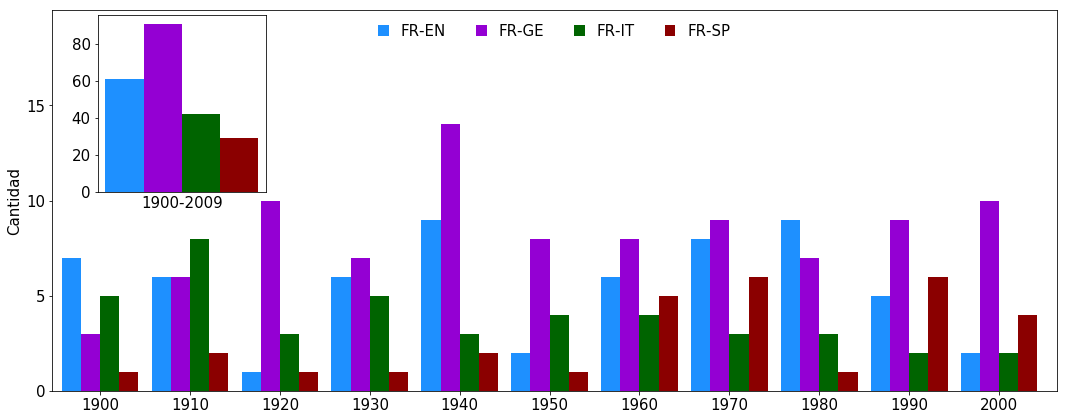
\includegraphics[scale=.38]{NC_FR.png}
	\label{fig.NC_FR}
	\caption{Palabras nuevas del francés hacia los demás idiomas. Entre las demás lenguas romances, el aporte del francés ha sido minoritario siendo las lenguas germánicas donde el francés asentó más elementos, descantado el alemán en las décadas durante la primera (1920) y segunda guerra mundial (1940).}
	
	
\end{figure}

\subsubsection*{Francés-Inglés}% {{{

La característica de los prestamos, es que son mayormente palabras  comunes en el ingles, y que podrían ser  catalogados como errores de clasificación, por ejemplo  \textit{diagnostic,} \textit{clients,} \textit{placement,} \textit{adaptation,} \textit{diffusion,} \textit{amplitude,}.  No pareciese lógico ver que estas palabras migraron del francés hacia el inglés, sin embargo el algoritmo designó este origen por ser al principio de la base de datos (1740)  donde las palabras eran más utilizadas.  



% }}}
\subsubsection*{Francés-Alemán}% {{{

El alemán tuvo dos décadas donde la cantidad de palabras nuevas que llegaron a él es más significativa que en los otros idiomas; entre 1920 y 1940  (años cercanos a las dos guerras mundiales), se ubicaron a  textit{diplomatie} (1917), \textit{bourgeoisie} (1919),  \textit{guerre} (1925), \textit{Allemagne} (1925), \textit{Russie} (1925) y \textit{empire} (1937); siendo un conjunto de palabras referentes a temas políticos  o diplomáticos acordes a las guerras. 


% }}}
\subsubsection*{Francés-Italiano}% {{{

El italiano se vio mas susceptible al francés en los primeros años del siglo, aunque no fue posible ligar  las palabras a un hecho relevante en estos años. Entre las pocas clasificaciones se encuentra el campo científico con \textit{Poincaré} (1924), apellido del matemático francés Henri Poincaré, y los campos bélico y político, con \textit{Versailles} (1924), \textit{Vietnam} (1966)  y \textit{URSS} (1975);  estos préstamos muestran a la primera y segunda guerra mundial como detonantes para el flujo de palabras.


% }}}
\subsubsection*{Francés-Español}% {{{

Al igual que la tendencia en el italiano, en el español hay pocas palabras cuyo contenido sea ligado a un evento. El termino más destacado fue \textit{euros} (2002) por ser el año de circulación de la moneda de la unión europea, organización donde son miembros España y Francia. 

%El hecho de no poder enlazar palabras a eventos, no significa que el francés no es importante para el español (o el italiano), sino que el periodo donde los hechos tuvieron mayor impacto no esta dentro del periodo de búsqueda,  por ejemplo hechos como la revolución francesa, o la invasión napoleónica a España, propiciaron a un mayor intercambio en este sentido, pero al ocurrir antes de 1900 no permite tener una conclusión de ello. 


% }}}
% }}}
\subsection{Alemán}% {{{

\begin{figure}[h!]
	\centering
	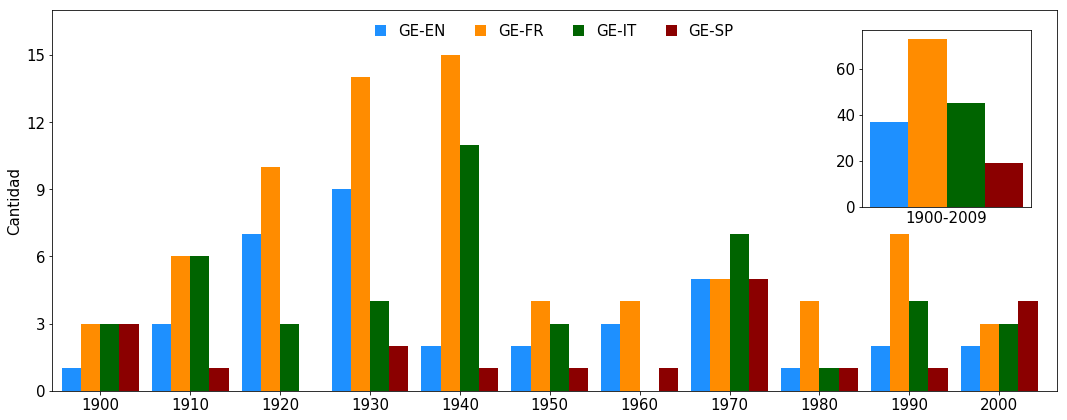
\includegraphics[scale=.38]{NC_GE.png}
	\label{fig.NC_GE}
	\caption{Palabras nuevas del alemán hacia los demás idiomas. El francés destaca durante la primera mitad del siglo como el idioma donde tiene más presencia el alemán, logrando las mayores migraciones en los años entre las guerras mundiales (1930-1940). Se distingue al español como el idioma con menos préstamos, existiendo décadas donde el aporte fue nulo.}
\end{figure}




\subsubsection*{Alemán-Inglés}% {{{

Como en la relación en sentido inverso, en los años posteriores a la segunda guerra mundial, se encontraron palabras ligadas al evento como  \textit{Lenin} (1931), \textit{Hitler} (1934) y \textit{reich} (1939).  Otras palabras relevantes son \textit{Marx} (1934) y \textit{Freud}, apellidos de dos personaje destacados en la filosofía y psicología. 


% }}}
\subsubsection*{Alemán-Francés}% {{{

%El francés ha recibido más palabras del alemán que cualquier otro. A pesar de que la mayor cantidad de aportes se dio en la primera mitad de siglo, las relaciones que se encontraron han sido a lo largo de todo el periodo y en diferentes áreas. 

Las migraciones son constantes en todo el siglo XX, destacando la década de 1940, con palabras como \textit{regierung}, \textit{deutschen},\textit{minister} y  \textit{bestimmungen}(traducciones de gobierno, alemán, ministro y reglamentos) todas apareciendo en 1944;  si se añaden palabras en años previos como \textit{Hitler} (1933), \textit{kaiser} (1915) y \textit{reich} (1921), son conceptos que muestran parte de la historia del alemán en las guerras. 

Una gran parte de las palabras nuevas son apellidos de  personajes nacidos en países germanohablantes,  además de Hitler se encontó a \textit{Nietzsche} (1905),  \textit{Marx} (1923), \textit{Heidegger} (1987),  \textit{Mozart} (1956), \textit{Freud} (1965) y \textit{Engels} (1970), enlazados a la filosofía, la música y la medicina. 


% }}}
\subsubsection*{Alemán-Italiano}% {{{

La característica principal de los prestamos que toma el italiano son personajes cuya lengua es el alemán,  además de los mencionados previamente, el único apellido que llegó exclusivamente al italiano fue \textit{Berchtold} en 1943, refretente a Leopold Berchtold ministro de exteriores del Imperio Austro-Húngaro de 1912 a 1915, cuyo fallecimiento ocurrió en 1942.


  
% }}}
\subsubsection*{Alemán-Español}% {{{

Las palabras que van en este sentido,  presentaron  décadas  con pocas migraciones. Destacan  \textit{Marx} (1932), \textit{kaiser} (1938), \textit{Hitler} (1940), \textit{Lenin} (1970), \textit{Hegel} (1971),  \textit{Nietzsche} (2000) y \textit{Freud} (2002).  Es peculiar que apesar de ser terminos que se encuentran en los otros idiomas, su aparicion en el español ocurrio  años despues que en los demás, por ejemplo en el francés,  Nietzsche apareció 1905 y Freud en 1965. El letargo de años puede ser una característica del tiempo que les lleva  a las  palabras del alemán pasar hacia el español, al adaptarse a una lengua de una familia distinta.





% }}}
% }}}
\subsection{Italiano}% {{{

\begin{figure}[h!]
	\centering
	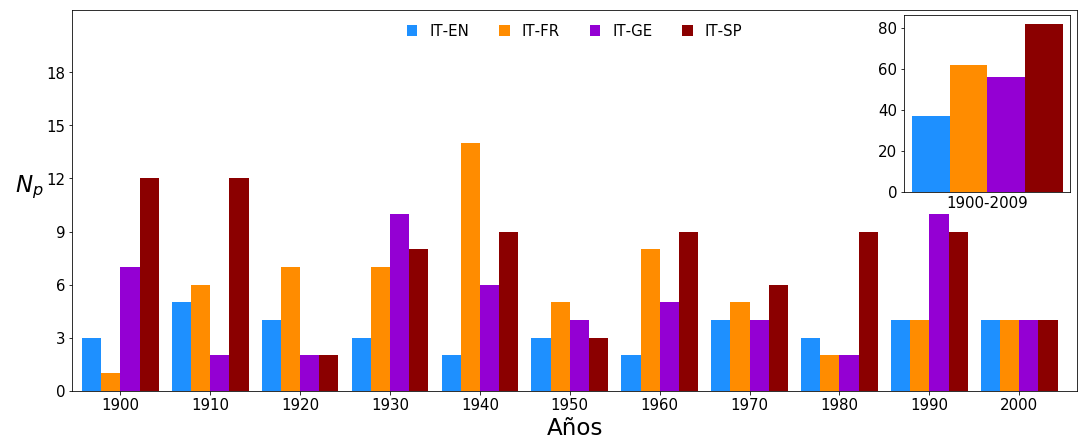
\includegraphics[scale=.38]{NC_IT.png}
	\label{fig.NC_IT}
	\caption{Palabras nuevas del italiano hacia los demás idiomas. Al provenir de la misma familia grecolatina y ser fonética y etimológicamente similares, el español y el francés han adoptado la mayor cantidad de palabras provenientes del italiano.} 
\end{figure}




\subsubsection*{Italiano-Inglés}% {{{

A pesar de que en cada década existen términos nuevos en el inglés, solo ha sido posible asociar \textit{mussolini} (1935),  alusivo al político y militar Benito Mussolini, quizá el personaje italiano más relevante para la historia en el siglo XX .

% }}}
\subsubsection*{Italiano-Francés}% {{{



En las migraciones sólo se asoció \textit{Mussolini} (1935), la cual ya se había mencionado previamente. Aunque en 1940 migraron la mayor cantidad de préstamos, ninguno de ellos ha tenido contexto con los sucesos de esa época. 

Tras revisar las listas de migraciones con origen italiano  a los demás idiomas, Mussolini siempre se encuentra en todas las migraciones y en el mismo año ratificando la importancia de este término en la historia. 



% }}}
\subsubsection*{Italiano-Alemán}% {{{

En esta dirección de existen relaciones con el contexto bélico,  \textit{regime} (1938), \textit{panzer} (1941), \textit{duce} (1942),  traducciones de régimen, blindado y líder, además de \textit{Mussolini} (1935). 



% }}}
\subsubsection*{Italiano-Español}% {{{

En el español, además guerra, se ecnotraron nombres de ideologías políticas,  \textit{socialista} (1914), \textit{comunista} (1932), \textit{capitalismo} (1935), \textit{fascismo} (1937),  \textit{marxismo} (1963) y \textit{terrorismo} (1986). 



% }}}
% }}}
\subsection{Español}% {{{

\begin{figure} % {{{
	\centering
	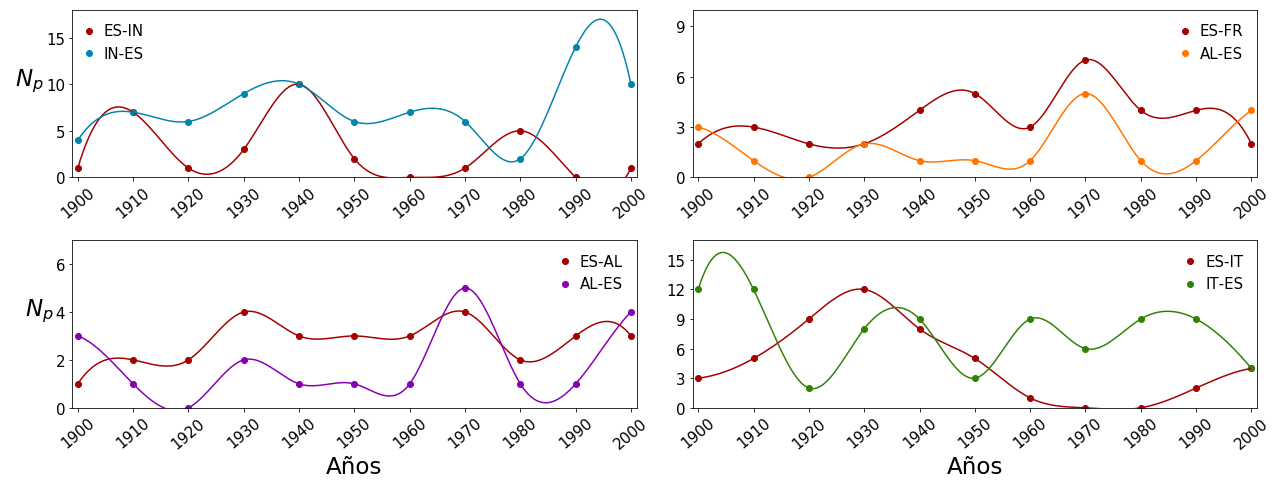
\includegraphics[scale=.38]{NC_SP.png}
	\label{fig.NC_SP}
	\caption{Palabras nuevas del español hacia los demás idiomas. El italiano es el idioma  que más palabras recibió del español, seguido del francés. El provenir de una misma familia es un factor para que existan migraciones.}
\end{figure} % }}}

\subsubsection*{Español-Inglés}% {{{

Contrario a la tendencia en las anteriores migraciones donde la guerra era una constante, en este sentido se encontraron términos médicos,  en el año de 1943  aparecieron  \textit{virus} y \textit{anemia}; años antes en 1934 George Richards Minot, Parry Murphy y George Hoiyt Whipple, habían recibido el premio Nobel de medicina por su descubrimiento de la terapia de hígado para el tratamiento de anemias.   

Probablemente las palabras virus y anemia ya existían en el inglés años antes de 1943,  pero sólo hasta este año tuvieron la importancia para estar dentro de las cinco mil más utilizadas. Esto ejemplifica que hay eventos (como un premio internacional) que retoman palabras cuyo periodo de uso  ha disminuido,  para volverse importante y dispersarse en los demás idiomas.


\subsubsection*{Español-Francés}% {{{

El primer préstamo que ligado del español hacia el francés es \textit{Panamá} (1913), su trascendencia se debe a la inauguración del canal de Panamá en 1914, siendo una obra importante para el comercio de la época al conectar los océanos pacífico y atlántico, además el primer gobierno que impulsó económicamente la construcción del canal fue el francés, aunque su conclusión y administración pasó a los Estados Unidos.  




% }}}
\subsubsection*{Español-Alemán}


Los préstamos son nuevamente términos médicos, la palabra \textit{lepra} (1901) fue globalmente importante a partir de 1874,  ya que en ese año el científico noruego Gerhard Armauer Hansen descubrió el bacilo de Hansen Mycobacterium Leprae \cite{lepra} que origina la enfermedad. Por el carácter médico de la palabra, es probable que se hiciera más investigación sobre la enfermedad en diferentes idiomas, en este caso el alemán. 


% }}}
\subsubsection*{Español-Italiano}% {{{

Los términos médicos han sido una constante en las migraciones del español, en el italiano se encontraron \textit{virus} (1922), \textit{colesterina} (1928),  \textit{sintomatología} (1931), \textit{anestesia} (1932), \textit{vitamina} (1935), \textit{anemia} (1936), \textit{metabolismo} (1936),  \textit{gástrica} (1936)  y \textit{endovenosa} (1937).  

El aparecer estas palabras en el español (dentro de las cinco mil más usadas)antes que en los demás,  sugiere que la medicina era un campo importante para los países de habla española, donde posiblemente se publicaron más libros de medicina en esta lengua. 






% }}}
% }}}
% }}}
\section{Comentarios del método}% {{{



Tras las múltiples combinaciones entre idiomas, se  encontró que el principal evento que origina las migraciones del siglo XX, ha sido la segunda guerra mundial, donde todos los lenguajes recibieron un termino asociado a ella.

Cada idioma se muestra como un portador de palabras de ciertos campos,  el inglés en economía, tecnología y política, el español en mediciona y el francés, el alemán y el italiano en la guerra.  Las areas mencionadas no dan una respuesta sobre que idioma ha sido más influyente, pero si muestra en que campos un idioma ha influido más que los otros, siendo esta una manera alternativa de hablar de influencia en los idiomas.
 
Una manera diferente de estudiar a los préstamos nuevos, sería midiendo el tiempo que le toma a las palabras moverse de un idioma a otro, dando una idea de la velocidad con la que migran. Aunque estos resultados pueden ser complementarios, por el momento no se han tratado. 


aunque por el momento este estudio no se ha tratado. 

%El inglés se presenta en las últimas dos décadas como el idioma común para transmitir información, exportando términos comunes en ámbitos como  la globalización y el desarrollo  de la tecnología.  Destaca el rol de los Estados Unidos como un país involucrado en los principales acontecimientos que originaron las migraciones, siendo usuales los apellidos de todos sus presidentes (posteriores a la segunda guerra mundial) en los demás idiomas. 

%Salvo el inglés que fue exportador en distintas áreas, los demás idiomas se caracterizaron por brindar palabras especificas,  el alemán por apellidos de personajes, el español por términos médicos, mientras que el francés y el italiano por la historia bélica y la religión. . 

 %Estos posibles resultados ayudarían a complementar la relación entre eventos, ya que en algunos eventos las palabras asociadas a él, migraron a los demás idiomas  en el mismo periodo, por ejemplo,  las palabras que migraron tras la revolución francesa (1789-1799) aparecieron en los diferentes receptores mientras ocurría el suceso y hasta veinte años después de él; así mismo,  los términos involucrados en la globalización  posterior a 1980 migraron en los años inmediatos a su invención.  Para tales complementos se necesitaría separar a los préstamos por áreas, lo cual no se hizo en este trabajo.  












% }}}



